\chapter{Instrumentation} \label{chp:instrumentation}
\section{Introduction} \label{sec:instrumentation/introduction}
Flexible and efficient instrumentation is the foundation of this project. Here, possible approaches to this instrumentation are discussed, along with critical analyses.

There are two main approaches to the instrumentation: automatic, and manual. 

\section{Automatic Approaches} \label{sec:instrumentation/automatic}
	In this context, an automatic approach to instrumentation is a technique that can be applied directly at compile-time (or just before run-time in an agent-like fashion). Such approaches require no human intervention whatsoever, and have the additional advantage of having access to additional compile-time meta-data which is not possible to gain at run-time or using manual instrumentation.

	\subsection{Graal} \label{sec:instrumentation/graal}
	In the first instance, an automatic approach based on Graal was investigated. Graal was chosen in the first instance because it is the most flexible approach: it allows the combination of compile-time evaluation, as well as run-time evaluation of the dependency algorithms.
	
	As mentioned, Graal uses various different forms of intermediate representation, based on graphs (see section \ref{sec:graal/ir}). In principle, it should be possible to modify these graphs in order to invoke the instrumentation (described in chapter \ref{chp:runtime}).
	
	Modifying graphs in Graal is made easy through a simple API. A user can define custom phases (see section \ref{sec:graal/transformations}). Pseudocode for this is as follows:
	
	\begin{lstlisting}[caption=Sample code for adding a phase and manipulating a graph,label=list:graph-trans]
	// create the phase
	public class MyPhase extends Phase {
	    @Override
	    protected void run(StructuredGraph graph) {
	        // modify the graph
	        for (LoadIndexedNode node:
	            graph.getNodes(LoadIndexedNode.class)) {
	            graph.addAfterFixed(node,
	                graph.add(new MyCustomNode()));
	        }
	    }
	}
	
	// add the phase
	Suites s = Graal.getRequiredCapability(SuitesProvider.class)
	    .createSuites();
	s.getHighTier().appendPhase(new MyPhase());
	\end{lstlisting}
	
	The call to \texttt{getHighTier()} can be replaced with equivalent methods for the other IRs (\ie, \texttt{getLowTier()} and \texttt{getMidTier()}.
	
	As we can see in figure \ref{fig:access-index}, which displays the high-level graph for a simple method that takes an array actual parameter and returns index $0$ of that array, there are specialised nodes for array accesses: \texttt{LoadIndexedNode}. Note that there is also an equivalent for array store operations, \texttt{StoreIndexedNode}.
	
	\begin{figure}[h]
		\centering
		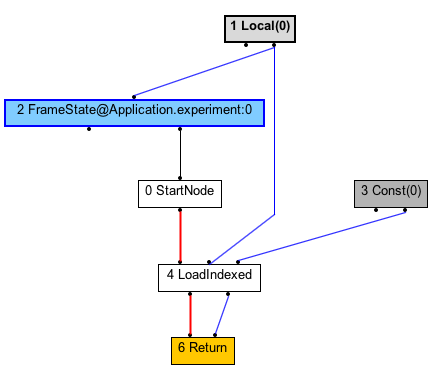
\includegraphics[width=.7\textwidth]{graphics/access-index.png}
		\caption{A high-level graph (with inlining disabled) for a simple method taking an array actual parameter, returning index 0}
		\label{fig:access-index}
	\end{figure}
	
	This is the basis for selecting the appropriate nodes to instrument. One additional advantage of Graal is the richness of the information available at compile-time. Figure \ref{fig:graal-meta} shows all the available information, as seen in Eclipse's debugger.
	
	\begin{figure}[h]
		\centering
		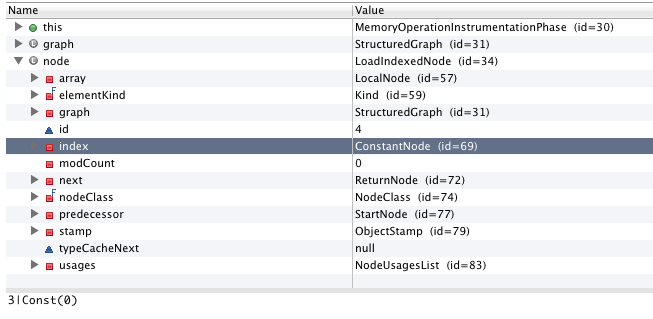
\includegraphics[width=0.8\textwidth]{graphics/graal-metadata.png}
		\caption{Information available at compile-time for the \texttt{LoadIndexedNode} shown in figure \ref{fig:access-index}}
		\label{fig:graal-meta}
	\end{figure}
	
	The availability of predecessor and next nodes, as well as nodes representing indexes (in this case, a \texttt{ConstantNode}) highlights another advantage of using Graal for these transformations - static analysis is possible, which means that instrumentation can be disabled if dependencies can be proven statically. 
	
	There are several possibilities for adding instrumentation in Graal.
	
	\begin{enumerate}
		\item \label{item:instr1} Add a custom node type, which is lowered to an invoke instruction after each applicable node.
	
		\item \label{item:instr2} Replace the nodes in question with a custom node that implements the same operation in addition to the required behaviour.
	
		\item \label{item:instr3} Javassist includes a method for replacing all array accesses with method calls \citep{JavassistDocs}. It may be possible to use Graal to replace the method call targets where instrumentation is required. In cases where no instrumentation is required, the method would return the array value (or perform the store), which would then be inlined by the compiler.
	\end{enumerate}
	
	In cases \ref{item:instr1} and \ref{item:instr2}, then node would need to implement \texttt{Lowerable}, an interface in Graal that allows nodes to be lowered between IR levels.
	
	\textit{However}, there is currently a limitation in Graal which means that it is not currently possible to insert calls to (static) methods. This is because there is no \emph{bytecode index} (or BCI) for the interpreter to return to if a deoptimisation occurs (details on Graal's deoptimisation mechanisms are available in section \ref{sec:graal/deopt}). Since methods calls cannot be guaranteed to be deoptimisation-free, they cannot be inserted into graphs. Any static methods that modify abstract data types (\ie, the storage formats described in section \ref{sec:runtime/storage}) cannot be assumed to be deoptimisation free. Modifying a data structure violates the optimisation assumptions, causing a deoptimisation. The interpreter then tries to resume from the BCI of the invoke. However, there is no BCI associated with inserted invocation, meaning that the interpreter cannot resume in the event of the inevitable deoptimisation. The end result is that insertation of arbitrary behaviour through invoke nodes to static methods is not currently possible in the Graal system.
	
	To illustrate the concept of BCIs, consider the following example. In Java bytecode, each instruction has an associated index (this example was compiled using \texttt{javap -c} from a basic `hello, world!' application):
	
	\begin{verbatim}
	Compiled from "Hello.java"
	public class Hello {
	  public Hello();
	    Code:
	       0: aload_0       
	       1: invokespecial #1    // Method java/lang/Object."<init>":()V
	       4: return        
	
	  public static void main(java.lang.String[]);
	    Code:
	       0: getstatic     #2    // Field java/lang/System.out:Ljava/io/PrintStream;
	       3: ldc           #3    // String Hello, world
	       5: invokevirtual #4    // Method java/io/PrintStream.println:(Ljava/lang/String;)V
	       8: return        
	}
	
	\end{verbatim}
	
	We can clearly see the BCIs of the various operations: the \texttt{invokespecial \#1} has a BCI of 1, and so on.

	This is a limitation of the Graal platform. In the coming months, the Graal core developers are adding this required feature. Once the feature has been added, it is a simple modification (as the infrastructure has already been created) to add this into Graal. Indeed, the required infrastructure for this transformation has been created -- once the support for it is available, only would need to enable the transformations.
	
	As an alternative, we used manual instrumentation (section \ref{sec:instrumentation/manual}). Although this does have the disadvantage of requiring both source-code access as well as human effort, this will not affect the results or correctness of the evaluation as the semantics are equivalent. The results and conclusions of this report will not be affected by this shortcoming of Graal. The required framework and infrastructure has already been developed, the mechanism through which the framework is used cannot affect the results in this case.
	
\section{Manual Approaches} \label{sec:instrumentation/manual}
The major alternative to automatic instrumentation is manual instrumentation, where the user manually performs the required transformations in the source code.

These transformations consist of replacing array access and store operations with method calls, whilst adding relevant metadata if required. For example, consider the following array access:

\begin{lstlisting}[label=list:array-access,caption=Standard array access in Java]
int c = a[b];\end{lstlisting}

Manual instrumentation refers to replacing this operation, and all such operations, with the following (or equivalent):

\begin{lstlisting}[label=list:instrumented-array-access,caption=Instrumented array access]
int c = access-array(a, b);\end{lstlisting}

The \texttt{array-access} method (and the implied \texttt{array-store} method) performs the dependency checking algorithms using the techniques as described in section \ref{sec:runtime/analysis/online}.
	
\section{Summary} \label{sec:instrumentation/summary}
In this section, we have considered the use of Graal for automatic instrumentation. We have seen that, due to a limitation in the current version of Graal, it is not possible to add arbitrary static method invoke instructions. Regardless of this limitation, there are other possible approaches that could also (in principle) be used for automatic instrumentation.

Lastly, we have seen how manual instrumentation is possible, and the reasons why the alternative approach used (manual instrumentation) will not affect the results or conclusions of this dissertation.